\graphicspath{{figures/tracking/}}

\section{Tracking the drone} \label{sec:TrackingTheDrone}
It was found in the preanalysis (\autoref{sec:ConclusionWPT}), that the \gls{wpt} is directional therefore the power transmitter on the ground station needs to be pointing directly at the power receiver on the drone. In order to point the motorised antenna stand in the right direction, the direction of the drone is needed. 

To describe the position of a drone flying in the air relative to the base station (the antenna stand), a spherical coordinate system is introduced. A point is space is associated with a distance from the origin to the point, $r$, an azimuth angle, $\phi$ and an elevation angle which is the angle between the origin, the point and the positive z-axis, $\theta$ \citep{book:calculus}. This is illustrated in \autoref{fig:spherecoords}.
\begin{figure} [h!]
\centering
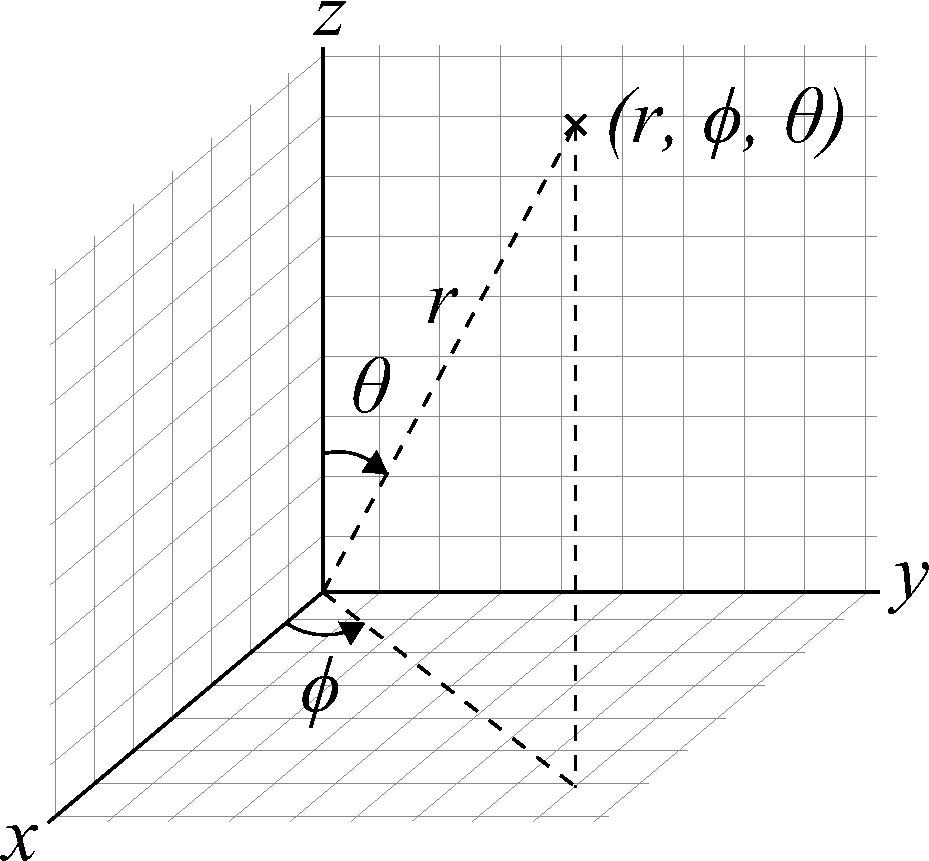
\includegraphics[width=0.4\linewidth]{3D_Spherical}
\caption{Spherical coordinates of a point in space \citep{website:spherecoords}.}
\label{fig:spherecoords}
\end{figure}

Once $\phi$ and $\theta$ are acquired this is sufficient to point the antenna is the right direction.
Several methods for measuring and determining $\phi$ and $\theta$ are investigated in this section. 
Before starting to research different methods of tracking the drone, the required precision of the tracking is determined. Now that the required precision is known and the the coordinate system is defined different tracking methods are studied.
\begin{itemize}
\item Optical tracking
\item \glsentrylong{aoa} determination from signal distance difference
\begin{itemize}
\item Time of arrival 
\item Phase difference detection 
\item Signal strength difference
\end{itemize}
\item GPS 
\item Radar
\end{itemize}

\subsection{Optical Tracking}
It is possible to locate an object using an optical sensor. This work by converting a change in light into a electric signal, that is measured and compared to a reference signal. 

Because of weather related issues, optical tracking of a drone might not be a functional solution. If the drone is behind clouds or simply is unrecognizable by the optical sensor, due to weather conditions like rain, snow or a fog, the optical tracking is not working. 

Because of these issues optical tracking is rejected. 

\subsection{\glsentrylong{aoa} determination from signal distance difference}\label{sec:detSignalDistanceDifference}
Signal difference is based on the fact, that if the drone is sending out a beacon signal, the distance the signal has to travel to reach two  different antennas on the ground is different. This difference in distance can be used to determine the \gls{aoa} of the signal. This signal difference can be determined in many different ways, in this subsection three different methods is explained and later in \autoref{subsec:SignalStrengthPathLossMethod} a third method is explained as well. 

All the methods using signal difference need a setup with two or more receiving antennas. For simplicity two antennas receiving setup is assumed in order to explain the functionality of the different methods. Such a receiver setup is seen on \autoref{fig:RSSI_tracking}. 
\begin{figure}[h]
	\centering
	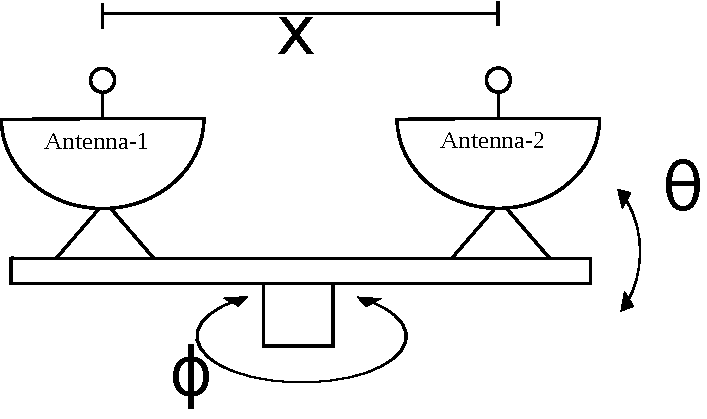
\includegraphics[width=0.6\linewidth]{AntennaSetupSeenFromAbove}
	\caption{Placement of tracking antennas in a signal difference tracking system, seen from above.}
	\label{fig:RSSI_tracking}
\end{figure}

The formula for determining the \gls{aoa} can be derived using geometry.
Considering a signal sent from the drone at point $P$ on \autoref{fig:phase_drawing}, two antennas are placed at respectively at $S_1$ and $S_2$. The paths that the signal travels to reach the two antennas are $d_1$ and $d_2$. At the point $M$ the signal has travelled the same distance.
The difference in length the signals have to travel is denoted $y$ and is equal to $d_1-d_2$. 
\begin{figure}[h]
\centering
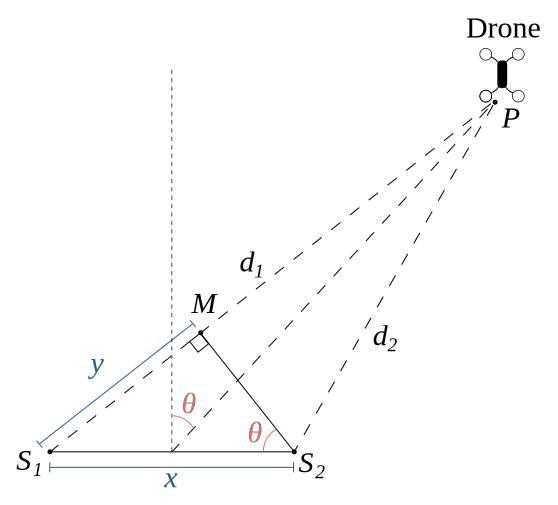
\includegraphics[width=0.7\linewidth]{Phase/Phase_drawing}
\caption{Illustration of determination of \gls{aoa} using signal distance difference. P is the point where the drone is located. $d_1$ and $d_2$ are the respective distances between the drone and the two receiving antennas $S_1$ and $S_2$. The distance between the antennas is $x$ and the difference of $d2$ and $d_1$ is y. $M$ denotes the point where the two distances are equal. The \gls{aoa} is approximately $\theta$ when $d_1 \gg x$ and $d_2 \gg x$.}
\label{fig:phase_drawing}
\end{figure}

The \gls{aoa}, $\theta$, can be calculated using trigonometry. It is assumed that the sender $P$ is so far away, so that from the two antennas point of view the drone is a plane instead of a point. This allows the approximation that the two lines, $d_1$ and $d_2$, can be considered parallel.
This means that the angle $\theta$ at $S_2$, also becomes the \gls{aoa} which can be calculated using sine \citep{TechReport:DirectionFindingPaper}.

The \gls{aoa} can then be calculated with \autoref{eq:aoa_general}. 
\begin{equation} \label{eq:aoa_general}
	\theta = \arcsin\left(\frac{y}{x}\right) \addunit{\radian}
\end{equation}
\startexplain
\explain{$\theta$ is the \gls{aoa}}{\si{\radian}}
\explain{$y$ is the physical distance difference, between each of the receivers and the drone}{\si{\meter}}\explain{$x$ is the spacing between the two antennas}{\si{\meter}}
\stopexplain

The method described above is only be able to measure \gls{aoa} within a \SI{180}{\degree} field of view since two mirrored points result in the same distance, $y$. 
This can be seen on \autoref{fig:phase_double}. To avoid this ambiguity, $y$ has to be measured with more than two receivers \citep{TechReport:Amundson2010}. In this report for the sake of simplicity only a two antennas setup is considered.
\begin{figure}[h]
\centering
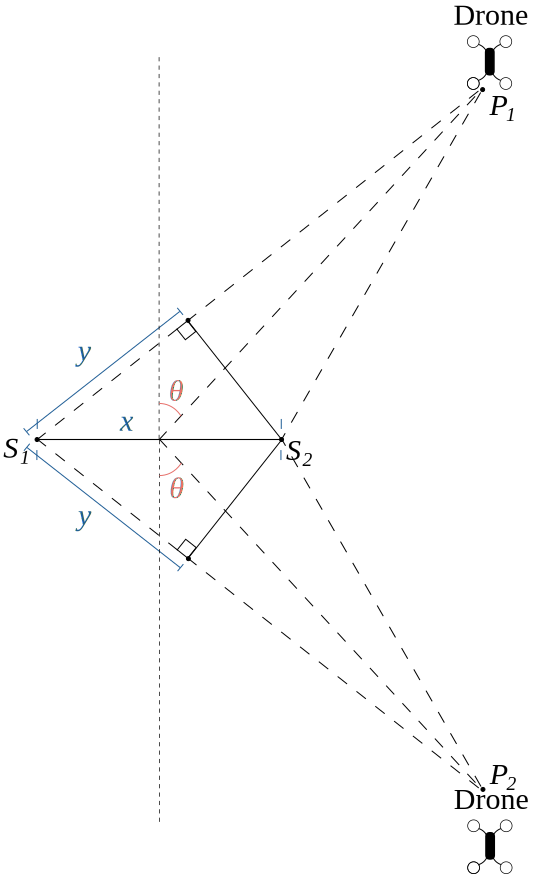
\includegraphics[width=0.4\linewidth]{Phase/phase_double}
\caption{The two points $P_1$ and $P_2$ result in the same signal characteristics being measured at the receivers $S_1$ and $S_2$. This means that a two antenna system only have a field of view of \SI{180}{\degree}}.
\label{fig:phase_double}
\end{figure}

\newpage
Three method using \gls{aoa} is analysed in this report:
\begin{itemize}
	\item Time of arrival 
	\item Phase difference detection 
	\item Signal strength difference
\end{itemize}

\subsubsection{\glsentrylong{toa}} \label{TimeOfArrival}
With this method a receiver setup as the one explained on \autoref{fig:RSSI_tracking} is assumed. In this case the drone emits a impulse signal whenever the position of the drone is needed. If the drone moves, a new impulse must be emitted in order for the ground station to know the new location of the drone.

The \gls{toa} method uses the time difference in reception of a source between two receivers. The finite speed of electromagnetic wave propagation causes a time difference between the reception time on two antennas when the signal source is not placed at exactly the same distance to each antenna.

The difference of time between the moment each antenna receives the signal multiplied with the speed of light, represents the difference in distance between the drone and each of the two antennas. That way the distance difference, $y$ from \autoref{eq:aoa_general}, can be determined by: 
\begin{equation} \label{eq:LenghtDifference}
		y = \Delta t \cdot c \addunit{\meter} 
\end{equation}
\startexplain
\explain{$\Delta t$ is the time difference between the two antennas reception of the signal}{\si{\second}}
\explain{$c$ is the speed of light}{\si{\meter \per \s}}
\stopexplain

Combining \autoref{eq:LenghtDifference} and \autoref{eq:aoa_general} yields \autoref{eq:actualLenghtDifference}. 
\begin{equation} \label{eq:actualLenghtDifference}
	 \theta = \arcsin \left( \frac{ \Delta t \cdot c}{x} \right) \addunit{\radian}
\end{equation}

If the difference in time is not registered and measured correctly the calculated angle deviate from reality. In \autoref{sec:RequiredPrecision} it was found that the allowed error in the tracking should be less than \SI{2,08}{\milli\radian}. By inserting the value of the allowed error combined with the assumption that the distance between the antennas is 20 cm into \autoref{eq:actualLenghtDifference} yield: 
\begin{subequations}
\begin{align}
\theta &= \arcsin \left( \frac{\Delta t \cdot \SI{300 000 000}{\meter\per\second} }{\SI{200}{\milli\meter}} \right) =  \SI{2,08}{\milli\radian} \label{eq:TOA:eq3} \\
\Delta t &= \SI{1,3867}{\pico\second} \label{eq:TOA:eq4}
\end{align}
\end{subequations} 

From \autoref{eq:TOA:eq4} it is seen that a measuring error of \SI{1,3867}{\pico\second} equals to the maximum allowed angular deviation. From this it can be deduct that the signal at the two receivers should be sampled much faster than $\frac{1}{\tau_{error}} = \frac{1}{\SI{1.3867}{\pico\second} } = 721 \si{\giga\hertz}$

For this project a sampling frequency of more than \SI{721}{\giga\hertz} is not possible for a digital implementation, as such it was decided to not pursue the research further.

\subsubsection{Phase difference detection} \label{PhaseDifferenceDetection}
With this method a receiver setup as the one explained on \autoref{fig:RSSI_tracking} is assumed. For this method the drone should emit a continuous wave signal. 

The distance difference $y$ from \autoref{eq:aoa_general}, can be determined by measuring the phase difference of the signal at the two antennas. Thus the difference in distance can be expressed by \autoref{eq:phasedaoay}. 
\begin{equation} \label{eq:phasedaoay}
y=\frac{\lambda\cdot\Delta\varphi}{2\pi} \addunit{\meter}
\end{equation}
\startexplain
\explain{$\lambda$ is the wavelength of the signal}{\si{\meter}}
\explain{$\Delta\varphi$ is the phase difference of the signal between the two antennas}{\si{\radian}}
\stopexplain

When isolating \autoref{eq:phasedaoay} for $\Delta\varphi$ the equation becomes \autoref{eq:phasedaoayV2}. 
\begin{equation} \label{eq:phasedaoayV2}
\Delta\varphi=y \cdot \frac{2\pi}{\lambda} \addunit{\radian}
\end{equation}

In practice when measuring the phase difference of the two signals it falls in the interval: $-\pi<\Delta\varphi<\pi$. Therefore it can be seen from \autoref{eq:phasedaoayV2}, that $y$ must fall in the interval $\frac{-\lambda}{2} < y < \frac{\lambda}{2}$. This relation can be ensured if the distance between the antennas is $\frac{\lambda}{2}$. This avoids phase ambiguity \citep{TechReport:DirectionFindingPaper,TechReport:Amundson2010}. 

The maximum phase difference occur when the sender is located collinear with the receiver. If the \gls{aoa} is directly above the two receiving antennas, the phase difference is \SI{0}{\radian}.

From \autoref{eq:aoa_general} and \autoref{eq:phasedaoay} the \gls{aoa} when using the phase difference becomes as descried by \autoref{eq:GeneralPhaseDelayEquation}. 
\begin{equation} \label{eq:GeneralPhaseDelayEquation}
	\theta = \arcsin\left(\frac{\frac{\lambda\cdot\Delta\varphi}{2\pi}}{x}\right) \addunit{\radian}\\
			   = \arcsin\left(\frac{\lambda\cdot\Delta\varphi}{2\pi x}\right)\addunit{\radian}
\end{equation}
\startexplain
\explain{$x$ is the distance between the antennas}{\si{\meter}}
\stopexplain

Errors in the \gls{aoa} reading occurs depending on the \gls{snr} of the signal, this error is defined by \autoref{eq:phase_doa_error} \citep[p. 43]{book:shinohara}. 
\begin{equation} \label{eq:phase_doa_error}
\Delta\theta ' = \frac{\lambda}{\pi x \cos(\varphi) \sqrt{\text{SNR}}} \addunit{\radian}
\end{equation}
\startexplain
\explain{$\Delta\theta '$ is the error of \gls{aoa} estimation}{\si{\radian}}
\explain{SNR is \glsentrylong{snr}}{1}
\stopexplain

From \autoref{eq:phase_doa_error} it is clear that the spacing of the antennas should be as large as possible to achieve the lowest \gls{aoa} estimation error. The maximum possible distance is $\frac{\lambda}{2}$ as described earlier in this section.

\cite{TechReport:DirectionFindingPaper} defines a worst case \gls{snr} of their tracking system to be \SI{20}{\decibel} and a best case \gls{snr} of \SI{60}{\decibel}.


A required precision was found in \autoref{sec:RequiredPrecision} \autoref{eq:RequiredPrecision}, to be better when \SI{2.08}{\milli\radian}. This means that a \gls{snr} of \SI{20}{\decibel} is not tolerable. 
To calculate the lowest tolerable \gls{snr}, values are inserted into \autoref{eq:phase_doa_error} this yields that  the lowest tolerable \gls{snr} should be above \SI{46.7}{\decibel} to achieve a precision of \SI{2.08}{\milli\radian} based on the calculated in \autoref{eq:phase_reqsnr}.
\begin{subequations} \label{eq:phase_reqsnr}
	\begin{align}
	\text{SNR} 	&> 10 \log_{10}\left(\frac{\lambda^2}{\pi^2x^2\cos(\varphi)^2\theta_{min}^2}\right) \addunit{\decibel}\\
			    &> 10 \log_{10}\left(\frac{2}{\pi^2\cos(0)^2 \cdot (\SI{2,08}{\milli\radian})^2}\right) \si{\decibel}\\
			    &> \SI{46.7}{\decibel}
	\end{align}
\end{subequations}

The \gls{snr} is a measure of the signal strength of the received signal compared to the signal strength of the noise. 

The \gls{snr} can be increased if more antennas are used, therefore more precise \gls{aoa} estimations are usually made with an array of receivers \citep{book:shinohara}. Another way to increase the \gls{snr}, is simply to increasing the received signal strength by transmitting with more power. 

The phase detection method has good potential, but the precision depends on the received power. 

\subsection{Signal strength difference} \label{SignalStrengthDifference}
Another way to determine the \gls{aoa} of a drone is to have the target drone emit a signal, whenever it wants to be tracked. The pilot signal is captured with a two antenna setup like the one seen on \autoref{fig:RSSI_tracking}. The strength of the two received signal are compared and used to locate the drone. This is known as \gls{rssi} tracking. 

%Another way to determine the \gls{aoa} of a drone is to compare the strength of a pilot signal that the targeted drone emits when it wants to be tracked. This is known as \gls{rssi} tracking. 
%%Assuming the drone is transmitting a pilot signal, that is collected by a  minimum two tracking antennas, these antennas should have a physical distance between them.  
%The strength of the signal emitted by the drone should be captured in two or more antennas, in order to compare the the signals. The antennas should be have a physical distance between them. 

The signal strength difference can be used in different ways to track the drone, some of the methods is analysed in this section. 

\subsubsection{Continuous tracking with closed feedback loop controller}
One method to find the direction of the drone is to have a two antenna setup as on \autoref{fig:RSSI_tracking}. 
The two antennas should continuously measure the signal strength of the incoming signal. The difference in received signal strength between the two tracking antennas is compared and treated as an error signal in a closed loop feedback controller. 

The stand rotate according to the signal strength of the two antennas. If the signal is strongest on the left antenna, then the antenna stand would rotate left, and vice versa.

By having this continuous tracking the antenna stand rotate until the signal strength of the pilot signal is equally strong on both of the tracking antennas, which is the case when the antenna stand is pointing directly at the drone. 

The method is simple and precise enough for many uses. However to increase the precision many factors have to be considered, including the directivity of the tracking antennas, the gain difference between the antennas and the reflections. 

\subsubsection{Signal strength path loss method}\label{subsec:SignalStrengthPathLossMethod}
Another method to find the drone with the setup shown on \autoref{fig:RSSI_tracking}, is to map \gls{rssi} to distance using the path loss method. For this method the drone needs to emit a signal as well, but in this case the shape of the signal is not important, it could both be an impulse or a continuous wave.

It is known that the signal strength is decreasing as the wave front travels trough free space. The equation for free space path loss is \autoref{eq:SSLossPath}, which is also a simplified version of Friis Transmission Equation (assuming two isotropic antennas in free space without any gain).
\begin{equation} \label{eq:SSLossPath} 
L = 20 \cdot \log10\left(\frac{4\pi\cdot d}{\lambda}\right) \addunit{\decibel}
\end{equation}
\startexplain
\explain{$L$ is the path loss}{\si{\decibel}}
\explain{$\lambda$ is the wavelength of the signal}{\si{\meter}}
\explain{$d$ is the distance between the antenna and the drone}{\si{\meter}}
\stopexplain

The path loss can be calculated if the power transmitted and the power received is known as seen in \autoref{eq:simplepathloss}
\begin{equation} \label{eq:simplepathloss}
L = 10\log10\left(\frac{P_R}{P_T}\right)  \addunit{\decibel}
\end{equation}
\startexplain
\explain{$L$ is loss}{1}
\explain{$P_T$ is the transmitted power}{\si{\watt}}
\explain{$P_R$ is the received power}{\si{\watt}}
\stopexplain

With \autoref{eq:SSLossPath} the distance from the receiving antenna to the transmitting antenna can be found with \autoref{eq:SSLossPathDistance} (Note that this is the distance from the drone to one of the receiving antennas). 
\begin{equation} \label{eq:SSLossPathDistance} 
d = \frac{\lambda}{4\pi} \cdot 10^{\frac{L}{20}} \addunit{\si{\meter}}
\end{equation}

If the distance from the drone to both the receivers is known, then basic trigonometry can be used to find the direction of the drone. The needed trigonometric calculations is the same as the ones used to utilize the signal distance difference method in \autoref{sec:detSignalDistanceDifference}, therefore the \gls{aoa} can be determined from \autoref{eq:aoa_general}. 

With this method the distance difference, $y$ (seen on \autoref{fig:phase_drawing} and in \autoref{eq:aoa_general}), can be calculated from the difference in distance to the drone. This is done by inserting \autoref{eq:SSLossPathDistance} into \autoref{eq:SSLossPathAngle1} which yields \autoref{eq:SSLossPathAngle2}. 
\begin{align}
y &= | d_{a1} - d_{a2} | \addunit{\meter} \label{eq:SSLossPathAngle1} \\
  &= \frac{\lambda}{4\pi} \cdot \left| 10^{\left(\frac{L_{a1}}{20}\right)} - 10^{\left(\frac{L_{a2}}{20}\right)} \right| \addunit{\meter} \label{eq:SSLossPathAngle2}
\end{align}
\startexplain
\explain{$y$ is the distance difference from each of the antennas to the drone}{\si{\meter}}
\explain{$L_{a1}$ is the path loss of antenna 1}{\si{\decibel}}
\explain{$L_{a2}$ is the path loss of antenna 2}{\si{\decibel}}
\explain{$\lambda$ is the wavelength of the signal}{\si{\meter}}
\stopexplain

Combining \autoref{eq:aoa_general} and \autoref{eq:SSLossPathAngle2} yields the final equation:
\begin{equation} \label{eq:SSLossPathAngleFinal}
	\theta = \arcsin\left( \frac{\lambda}{4\pi \cdot x} \cdot \left| 10^{\left(\frac{L_{a1}}{20}\right)} - 10^{\left(\frac{L_{a2}}{20}\right)} \right|  \right) \addunit{\radian}
\end{equation}
\startexplain
\explain{$\theta$ is the \gls{aoa}}{\si{\radian}}
\explain{$x$ is the spacing between the two antennas}{\si{\meter}}
\stopexplain

In order for this method to work the fraction inside the arcsin should always be less than 1, as stated in \autoref{eq:SSLossPathAngleRule}, else the found angle becomes complex. 
\begin{equation} \label{eq:SSLossPathAngleRule}
\frac{\lambda}{4\pi \cdot x} \cdot \left| 10^{\left(\frac{L_{a1}}{20}\right)} - 10^{\left(\frac{L_{a2}}{20}\right)} \right| \leq 1
\end{equation}

If an error occurs and the signal strength is measured wrong, then the found \gls{aoa} is of course not exact.  Assuming a frequency of \SI{800}{\mega\hertz} and a distance between the antennas of \SI{20}{\centi\meter}. Then if the signal strength, in one of the antennas is measured with at error of \SI{3}{\decibel}, using \autoref{eq:SSLossPathAngleFinal} this means an error of \SI{691}{\milli\radian} in the found direction of the drone which is 300 times more that our allowed angular deviation. 



\subsection{\glsentryshort{gps}}
A commonly used system for location estimations are the \gls{gps}. \gls{gps} uses satellites to estimate speed and location, by utilizing the \gls{toa} method \cite{web:GPSUseTOA}. The \gls{gps} locator has to be placed on the drone and the coordinates have to be communicated wirelessly to the ground station.

The available drone (3DR Solo) has an integrated \gls{gps} module on-board, UBLOX Neo m7n. Users of this drone have 
experienced long satellite acquisition times, it usually takes 30 seconds to require a position on known area and up to one minute if the drone is flying in new areas \citep{datasheet:NEO7}. %The problem with this long satellite acquisition time is caused by the copper foil that are protecting the \gls{gps}. It may interferes with the electronic and can create shortcuts on the board if the copper foils isn't applied properly\citep{News:3DRGPS}. 

The precise accuracy of the \gls{gps} standard cannot be generalised, because its precision depends on many varying parameters. The U.S government however promises a worst case pseudorange (Pseudorange is the distance from the \gls{gps} satellite to the \gls{gps} device) accuracy of 7.8 meters at a 95\% confidence level, this means that the distance from a GPS satellite to a receiver have an accuracy of at least 7.8 meters for more than 95\% of the time \citep{web:USofAsGPSAccuracy}. 

The actual end user accuracy of the \gls{gps} is frequently being measured by the \gls{ffa}, their last tests show that the end user should normaly expect between 3-8 meters accuracy without the use of any augmentation systems. However in some cases, a range error of up to 23 meter was registered \citep{web:FFAGPSAccuracy}.

If the drone is \SI{120}{\meter} from the ground station, and the drones position is found, but with a deviation of 3 meters, that result in the angle of the motor stand have an error of $\theta = \arctan\left(\frac{3}{120}\right) = \SI{24.995}{\milli\radian}$. This means that the \glossary{gps} method is not meeting the required precision found in \autoref{sec:RequiredPrecision} \autoref{eq:RequiredPrecision}, and is therefore not feasible for the purpose of the project. 

If \gls{gps} is combined with some augmentation systems it is possible to have a higher accuracy. Examples of augmentation systems could be to use other wireless signals to position the user, such as wifi and cellular signals. 

With the limited and varying precision of the \gls{gps} method, it is not able to deliver the needed accuracy for this project, therefore the method is discarded, and is therefore not investigated further.  

\subsection{Radar}
When tracking objects an obvious mention is radar technology. Radars is used extensively around the world for geological observation, general surveillance and detection and tracking of flying objects such as airplanes and missiles \citep{radar_handbook}. 
Radar detection and tracking works by having a radar station transmitting a beam of microwave-frequency electromagnetic waves in the direction of an object. When the beam hits an object the waves are reflected back to the radar station. The time from transmission to reception is then used to find the distance to the target, and combined knowledge of the radars azimuth and elevatory heading the targets direction can be deduced, thus the target is located \citep{TechReport:RadarSystem}.

An illustration of a radar emitting a signal which is reflected upon a plane is seen on \autoref{fig:RadarMethodDrawing}. 
\begin{figure}[h!]
    \centering
        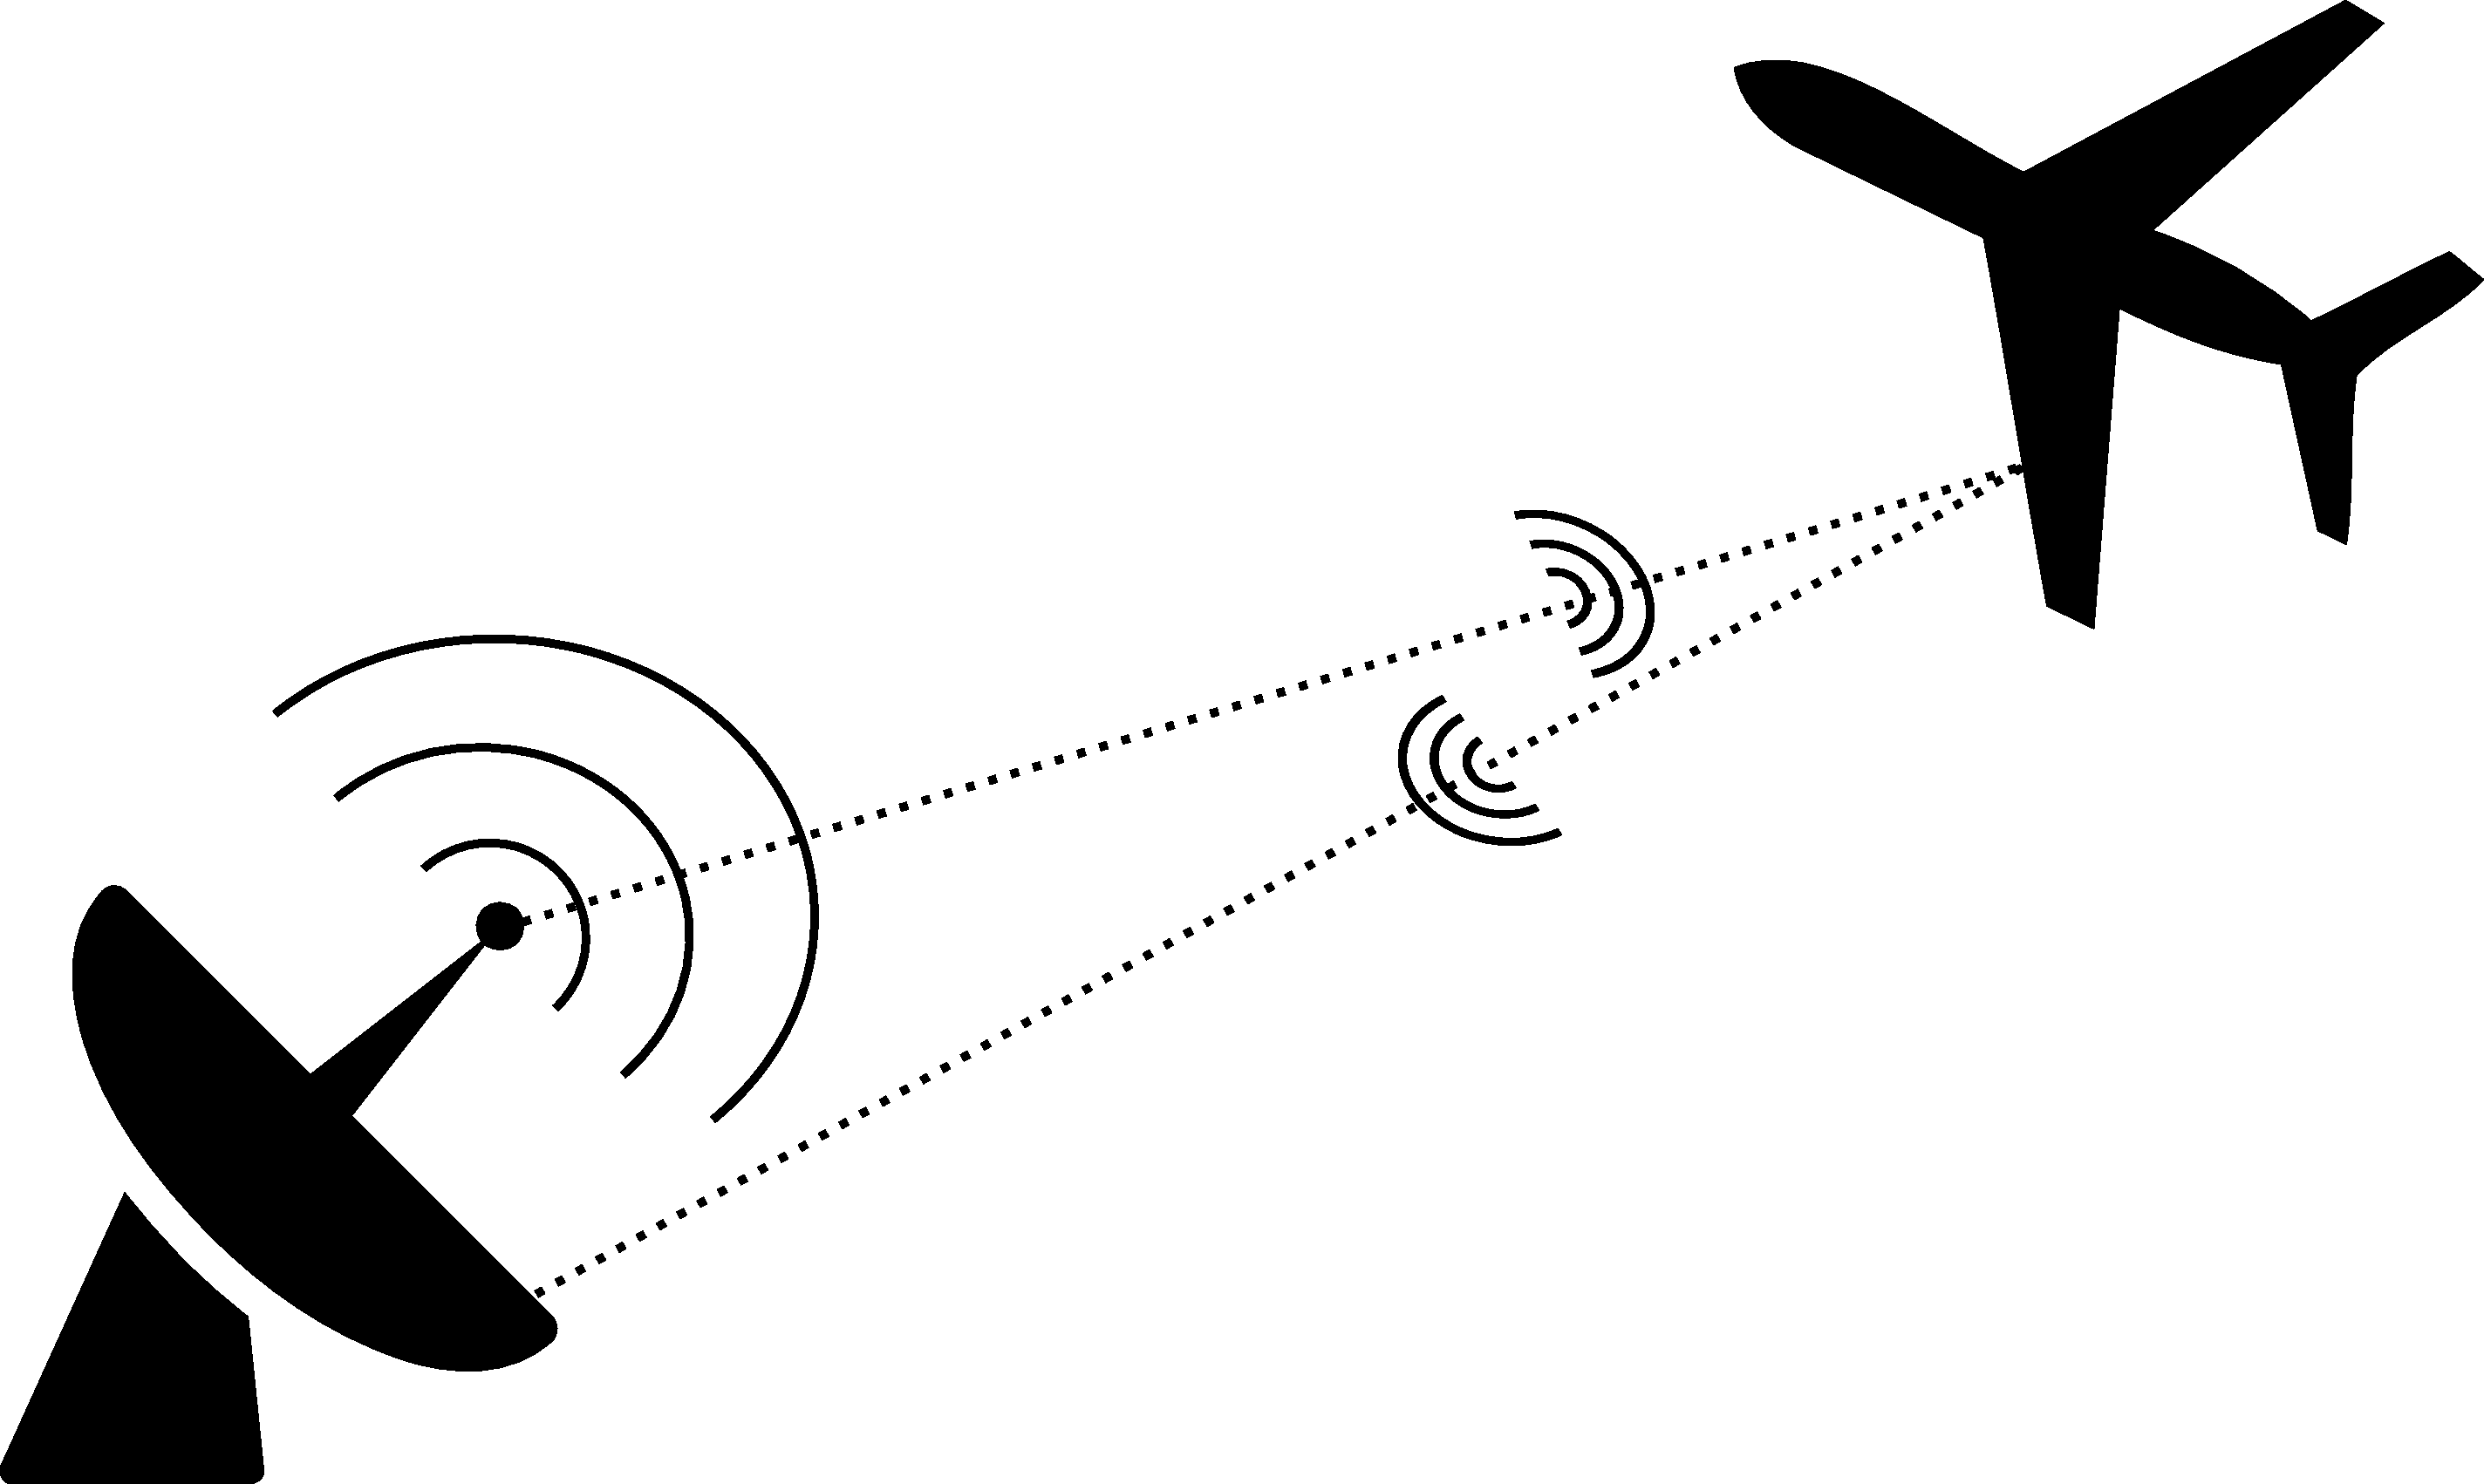
\includegraphics[width=0.5\textwidth]{figures/tracking/RadarMethodDrawing.pdf}
        \caption{The radar emitted an electromagnetic wave. The wave hits a plane, and is reflected back to the radar.}
        \label{fig:RadarMethodDrawing}
\end{figure}

\newpage
Many types of radar exists. When used for geological observation a wide beam is desirable, when used for aircraft or missile detection full $360\degree$ view is needed and when used for tracking a single targets speed and heading a very narrow beam is desired \citep{radar_handbook}.

\autoref{eq:Radar:ThinkItIsTheFrissGuyAgain} is the radar equation, it can be used to estimate the signal strength of the received reflections \citep{web:ThroughTheEyesOfARadar}. 
\begin{equation} \label{eq:Radar:ThinkItIsTheFrissGuyAgain} 
P_{r} = P_{t} \cdot  \frac{G_{r} \cdot G_{t} \cdot  \lambda^{2} \cdot \sigma}{(4\pi)^{3} \cdot R_{t}^{2} \cdot R_{r}^{2}} \addunit{\watt}
\end{equation}
\startexplain
\explain{$P_{r}$ is the power received}{\si{\watt}}
\explain{$P_{t}$ is the power transmitted}{\si{\watt}}
\explain{$G_{r}$ is the gain of the receiver antenna}{\si{1}}
\explain{$G_{t}$ is the gain of the transmitter antenna}{\si{1}}
\explain{$\lambda$ is the wavelength}{\si{\meter}}
\explain{$\sigma$ is radar cross-section (RCS)}{\si{\meter^2}}
\explain{$R_{t}$ is the distance between the transmitter antenna and the object}{\si{\meter}}
\explain{$R_{r}$ is the distance between the receiver antenna and the object}{\si{\meter}}
\stopexplain

\autoref{eq:Radar:ThinkItIsTheFrissGuyAgain} can be simplified by assuming that the receiver and the transmitter is the same antenna, and that it has a gain of 1.
\begin{equation} \label{eq:Radar:simplyfiedEquation1} 
P_{r} = P_{t} \frac{\lambda^{2} \sigma}{(4\pi)^{3} R^{4}} \addunit{\watt}
\end{equation}

By assuming a frequency of \SI{800}{\mega\hertz} and a distance between the antennas and the drone of \SI{120}{\meter} then \autoref{eq:Radar:simplyfiedEquation1} becoms: 
\begin{equation} \label{eq:Radar:simplyfiedEquation3} 
P_{r} = P_{t} \cdot \sigma \cdot 341.280 \cdot 10^{-15} \addunit{\watt}
\end{equation}

The radar cross-section of a drone is estimated to be between -10 to \SI{5}{\deci\belsm} (Where \SI{-10}{\deci\belsm} is the equivalent of a stealth military aircraft and \SI{5}{\deci\belsm} is a medium sized commercial aircraft) \citep{web:ThroughTheEyesOfARadar}. 

%Thus the radar cross-section, $\sigma$, of a drone is between $10\dfrac{-10}{11} = 0.1$ and $10\dfrac{5}{10} = 3.1623$

By including the radar cross-section of a medium sized commercial aircraft, to serve as a best case scenario in \autoref{eq:Radar:simplyfiedEquation2}, the received power can be calculated by \autoref{eq:Radar:simplyfiedEquation2}.
\begin{equation} \label{eq:Radar:simplyfiedEquation2} 
P_{r} = P_{t} \cdot 10^{\frac{5}{10}} \cdot 341.280 \cdot 10^{-15} = P_{t} \cdot 1.079 \cdot 10^{-12} \addunit{\watt}
\end{equation}

From \autoref{eq:Radar:simplyfiedEquation3} it is seen that if the used antenna does not have any gain, and if the target object has a radar cross-section of \SI{5}{\deci\belsm}, one needs to transmit approximately $10^{12}$ times more power than one needs to receive. 

If a received power of \SI{-20}{\deci\belm} is desired, \autoref{eq:Radar:simplyfiedEquation3} can be used to calculate the needed transmission power, as seen in calculated in \autoref{sec:radarRequiredPower2}
\begin{subequations}
\begin{align}  
P_{r} &= P_{t} + 10\cdot \log_{10}\left(1.079 \cdot 10^{-12}\right) \notag \\ 
P_{t} &= \SI{100}{\deci\belm} \label{sec:radarRequiredPower2}
\end{align}
\end{subequations}

The power needed decreases with increased gain. Using the exact radar cross-section of the target in question is probably mean a decreased efficiency, due to the radar cross section of the target being smaller than the assumed \SI{5}{\deci\belsm}. 

High gain antennas are needed in order for the radar method to work, because it is assumed that the required power levels described by \autoref{sec:radarRequiredPower2}, is not feasible for this project. Antennas with high a gain is outside the scope of this project and therefore this method is not possible for this project.

%with a limited transmission power of  the the needed gain can be found by looking back at \autoref{eq:Radar:ThinkItIsTheFrissGuyAgain}, as seen in \autoref{eq:RadarNeededGain}. 
%\begin{subequations}
%\begin{align} 
%&G_{r} \cdot G_{t} \cdot 1.079 \cdot 10^{12}\cdot P_t = P_r  \label{eq:ExplainNextEq}\\
%&\implies G_{r} \cdot G_{t} \cdot 1.079 \cdot 10^{-12} = 1 \label{eq:RadarNeededGain}\\
%&\implies G_{r} \cdot G_{t} = 0,927 \cdot 10^{12} \label{eq:RadarNeededGain3}
%\end{align}
%\end{subequations}
%
%\autoref{eq:RadarNeededGain3} can be simplified to \autoref{eq:RadarNeededGain2}, by assuming that $G_{r} = G_{t}$. \autoref{eq:RadarNeededGain2} calculates the needed gain for each of the two antennas. 
%\begin{align} \label{eq:RadarNeededGain2} 
%G_{r} \wedge G_{t} = \sqrt{0,927 \cdot 10^{12}} = 0.963 \cdot 10^6 \\
%G_{r} \wedge G_{t} = 10 \log10(0.963 \cdot 10^6) =  \SI{59,835}{\decibel}
%\end{align}

%As it is seen in \autoref{eq:RadarNeededGain2} the radar detection method needs two antennas with at very high gain. Antennas with this high a gain is outside the scope of this project and therefore this method is not possible for this project. 


\subsection{Conclusion on tracking metods}\label{sec:pre:trackingConclusion}
With all the different methods of tracking the drone investigated a conclusion is to be made. An overview of the conclusion of the different methods are seen in \autoref{tab:TrackingConclusion}.

Optical tracking is discarded as it is too dependent on environmental conditions to be effective.

Using radar technology to track different objects is already a widely used technique however it requires antennas with a high gain or high transmission power levels. The radar method is assessed to be too complex for this project.  

Despite of the inherent simplicity of the signal strength method it does not have the precision required.

Using the on-board \gls{gps} module on the drone to track it is a possible solution had the \gls{gps} been more precise. The \gls{gps} method might however be useful to generate rough estimate of the drones position if it is found needed. 

The time of arrival method shows great tracking potential, but to reach the wanted precision it becomes infeasible due to the need of high speed sampling.

The phase difference method shows many of the same characteristics as the time of arrival method, but without the need for high speed sampling.

\begin{table}[h!]
\centering
\caption{Summary of the different methods of tracking the drones direction.}
\begin{tabularx}{\textwidth}{l X }
	\textit{Method} 	& \textit{Summery} 	\\ \toprule \rowcolor{lightGrey}
	Optical tracking	& Too weather dependent 					\\
	Time of arrival		& Requires a high sampling frequency and sensitive electronics \\ \rowcolor{lightGrey}
	Phase difference 	& Good solution	\\ 
	Signal strength 	& Very noise prone and not precise enough \\\rowcolor{lightGrey}
	GPS					& Easy implemented, not very precise \\ 
	Radar & Complex, require high antenna gain\\
\end{tabularx}
\end{table} \label{tab:TrackingConclusion}

It is chosen to utilize the phase difference method to track the drone. The motorised antenna stand is now analyzed.



